\chapter{Robot Embodiment and Child Learning} \label{chap:embodiment}

\begin{framed}
	\textbf{Key points:}
	
	\begin{itemize}
	\item An experiment was designed to explore differences in child \gls{learning} and social behaviour in response to a physical robot, or a virtual robot (on-screen).
	\item A novel dataset was created for use as part of a category-based sorting game.
	\item The dataset used introduced a bias in the results, but this was accounted for.
	\item Results do not reveal any differences in \gls{learning} between the two conditions, but differences are found in children's social behaviour towards the robots. The physical robot attracts more gaze from the children than the virtual robot, demonstrating the promise of physically present social robots for dyadic tutoring.
	\end{itemize}
\end{framed}

Parts of the work presented in this chapter have been published in \cite{kennedy2014children} and \cite{kennedy2015comparing}\footnote{Note about technical contributions in this chapter: the author used software from the \acrshort{alize} project for the touchscreen, basic robot functionality for pointing at and selecting images on the screen, and low-level robot control. The author contributed the material used within the touchscreen software, some of the robot to touchscreen communication, the high-level robot social behaviour programming, and the porting of the robot software to the virtual robot.}. The final publications are available from Springer via http://dx.doi.org/10.1007/s12369-014-0277-4 and the ACM via:\newline http://dx.doi.org/10.1145/2559636.2559820

\newpage
As stated in Chapter~\ref{chap:background}, the application of social robots to the domain of education is becoming more prevalent. However, there remain a wide range of open issues, such as the effectiveness of robots as tutors on student learning outcomes, the role of social behaviour in teaching interactions, and how the embodiment of a robot influences the interaction. This chapter presents a study intended to explore children's behaviour towards a robot tutor for children in a novel guided discovery learning interaction. 

Chapter~\ref{chap:background} introduced literature relating to the embodiment of robots. It was suggested that the physical presence of a robot can have a large impact on human behaviour, possibly due to the social presence theory \citep{biocca2003toward} and a social facilitation effect \citep{triplett1898dynamogenic,zajonc1965social}. A positive effect of using a physical robot on performance has been shown in different task contexts with adults, including in a negotiation game \citep{bartneck2003interacting} and solving logic puzzles \citep{leyzberg2012physical}. However, with children, studies have shown no significant differences in learning \citep{westlund2015comparison}, do not control for prior knowledge \citep{han2008comparative}, or do not control for exposure time to material between embodiment conditions \citep{hyun2008comparative}. However, social behaviour responses of children have been observed due to differing robot embodiments \cite{looije2012help}. The positive effects observed with adults in addition to the social response of children to physical robots suggests that this is an area worth further experimentation.

To address this gap in the literature, the study in this chapter seeks to directly compare robot behaviour when instantiated on screen against on a physical robot. Prior knowledge and exposure time are controlled for. While constrained compared to that of the human, the robot tutor behaviour demonstrates sensitivity to the behaviour of the child, and emphasises the structured self-discovery of the subject matter to be learned by the child. A novel set of information for the children to learn was devised to ensure that the children involved would have no prior knowledge and so would start at the same experience level. There are two primary aspects of interest: firstly, whether the embodiment of the robot impacts on how much children learn, and secondly, how the children behave in the interaction in response to the tutoring strategy of the robot.

In many \acrshort{hri} studies there has been a focus on prescriptive tutoring, with the robot providing instructional lessons to subjects; a `teacher-centred' approach to learning, for example \citet{leyzberg2014personalizing}. However, educational literature suggests that a `learner-centred' approach confers many advantages; for example, learners can gain a deeper understanding of the material and can be more motivated due to an increased responsibility for their own learning \citep{spencer1999learner}. Such an approach is taken in \cite{kanda2012children}, for example, where children undergo collaborative learning with a robot in a variety of group and individual lessons.

The learner centred approach taken in this study, `guided discovery learning', has overlaps with the collaborative learning seen in \cite{kanda2004interactive}, but also some important differences. In collaborative learning, interacting partners are often peers. However in guided discovery learning, one of the interacting partners has more knowledge and can therefore guide the learner towards a correct solution. Learners must generate their own hypotheses, which they then test, and analyse the results, which uses skills that would not be developed when the necessary information is simply presented by a teacher \citep{de1998scientific}. It has also been suggested that this type of learning can promote a better understanding of a domain when compared to teacher-centred learning \citep{alfieri2011does, van1998cognitive}.

In a similar manner to collaborative learning, the teacher initially delivers enough instruction for problem solving to commence. However, instead of providing a lesson when learners get stuck, the teacher will help to guide the learner towards the correct solution by scaffolding analysis of the decisions the learner made surrounding hypothesis generation and analysis, with the aim of improving in the next ``hypothesis--test--analyse'' cycle \citep{de1998scientific, harvel2010guided}. Such an approach requires the robot behaviour to be responsive to the child not only in the task-related actions, but also in social behaviour. The robot needs to be sufficiently social to maintain the child's engagement throughout the interaction as the exploration is led by the child. The robot has key guidance for the child, and if they lose interest in the robot, then this could negatively impact their ability to succeed in the learning task. The robot behaviour must also be appropriate given the context, and to this end, a human model is used to derive the social behaviour; details are provided in Section~\ref{sec:ch6-meth-robobehave}.

The age of the subjects used in this experiment had to be carefully selected in order to make sure that the children had the cognitive skills to direct the exploration and motivate themselves to solve the problem presented. With the assistance of teaching professionals, it was decided to use children of around 8 years old. This age is quite novel in educational interactions, with most studies using subjects aged 10 and older (for example \citealp{kanda2012children, leyzberg2014personalizing, pereira2008icat, saerbeck2010expressive}). Since the necessity of real robots (as opposed to virtual agents) in education has not been definitively established in the literature, the effect of robot embodiment was assessed here. The aim of the experiment was to evaluate differences in child \gls{learning} and social behaviour in response to a physical robot, or a virtual robot (on-screen), i.e., the robot embodiment.

%%%%%%%%%%%%%%%%%%%%%%%%%%%%%%%%%%%%%%%%%%%%%%%%%%%%%
\section{Hypotheses} \label{sec:ch6-hypoth}
The purpose of the study conducted here was primarily to explore children's responses to robot behaviour across different embodiments in a novel guided discovery learning task. This means that the central hypotheses are based around the child's behaviour. Given that the interactions are educational, part of the validation also lies in how well the children learn, particularly with regards to differences between embodiments. Other work, such as \cite{looije2012help}, has found differences in gaze behaviour between embodiment conditions and it would be reasonable to predict that the same will be found in this study, despite substantial differences in context. Prior studies with a similar task structure and hardware configuration (robot with a large touchscreen), for example \cite{baxter2013emergence}, have found that the children will gaze more towards the touchscreen than the robot. However, if the robot behaviour is sufficiently social, then the children will remain engaged with the robot throughout the interaction. This can be examined through child responses to the robot's behaviour and activity in the task. Other studies have also found that the physical presence of a robot causes an increase in \gls{learning} gains, for example \cite{bainbridge2008effect, leyzberg2012physical}. Again, we predict the same effect here. From this background, the hypotheses derived for the study are enumerated below:

\begin{enumerate}
	\item [\textbf{H1:}] The real robot will attract more gaze than the virtual robot from the children. 
	\item [\textbf{H2:}] The children will remain engaged with both the robot and the task throughout the interaction.
	\item [\textbf{H3:}] Children will gaze more towards the touchscreen than the robot, but they will still pay attention to, and respond to, the robot's behaviour.
	\item [\textbf{H4:}] Children will exhibit greater \gls{learning} gains after interacting with a physically embodied robot. 
\end{enumerate}

%%%%%%%%%%%%%%%%%%%%%%%%%%%%%%%%%%%%%%%%%%%%%%%%%%%%%
\section{Experimental Setup}\label{sec:ch6-embodiment-setup}
The study design compares an Aldebaran NAO under two embodiment conditions: physically present and displayed virtually on a large screen. The conditions are employed in a between-subjects design. The study was informed by numerous pilot studies which explored the assessment of children's \gls{learning} when interacting with each other and an interaction mediator, the Sandtray touchscreen \citep{baxter2012touchscreen}. It was decided that the most appropriate task to assess \gls{learning} would be an adaptation of the sorting task with which several other experiments have been run \citep{baxter2013emergence, kennedy2013constraining}. Previous experience of using this task for \acrshort{chri} has led to the development of a practiced experimental protocol which serves as a solid foundation for use in this work.

\subsection{Participants}
Full permission to take part and be recorded on video was acquired for all participants. In total, 37 interactions took place, however, nine of these were not suitable for analysis. One child asked to stop before the interaction was completed, whilst in the other eight cases the experimental protocol was not followed. The breaks in protocol included technical issues with the robot/mediator, one child leaving to go to the toilet and one instance of Wizard error. As a result, 28 child-robot interactions were completed and recorded (11M, 17F, aged 7 or 8 years old, \textit{M}=7.9, \textit{SD}=0.31). 

A further two interactions could not be included in the learning assessment because an incorrect dataset was displayed, or logging did not complete correctly during either the pre- or post-test. 26 pairs of pre- and post-tests were analysed in terms of \gls{learning} and correlating social behaviour to learning outcomes (11M, 15F, age \textit{M}=7.9, \textit{SD}=0.33).

\subsection{Conditions}
The address the hypotheses, a two condition, between-subject design was employed for the study. The embodiment of the robot was swapped between the two conditions:
\begin{enumerate}
	\item A `real', physical Aldebaran NAO robot (\textit{n}=15 for interaction analysis; 14 for \gls{learning} assessment)
	\item A large monitor displaying the virtual robot, an Aldebaran NAO from the Choregraphe software (\textit{n}=13 interaction; 12 learning)
\end{enumerate}

The use of these two embodiment conditions allows evaluation of the experiment hypotheses, which all assume the presence of an agent (be it real or virtual) to interact with the child. The virtual robot acts as a control for the real robot, making it possible to explore the differences between the embodiments.

The robots in the two different conditions were made as close to the same size as possible (Figure~\ref{fig:ch6-embod}). It has been found previously that when children interact with a virtual robot with the same morphology as a physical robot that they have already interacted with, they can see this as the same character \citep{segura2012revive}. Although the children were interacting with the robot in only one of the embodiment conditions, there was a concern that their peers could tell them about the robot in the other condition. As such, the robots used were arbitrarily given different identities, using different gender-neutral names and different colours. The real robot had grey features and was named `Pop', whilst the virtual robot had blue features and was named `Crackle' (Figure~\ref{fig:ch6-embod}).

\begin{figure}[t!]
    \centering
    \includegraphics[width=0.9\textwidth]{images/ch6_RealVsVirtual_compressed.pdf}
    \caption{Side-by-side images of the  virtual (\textit{left}) and real (\textit{right}) robots used for this study: the Aldebaran Nao. The images are stills taken from one of the cameras used for filming. Scaling has been kept consistent between the two images so that size comparisons can be made.}
    \label{fig:ch6-embod}
\end{figure}

\subsection{Interaction Scenario}\label{sec:ch6-meth-setup}
The experiment took place in a primary school in the U.K. The room used was a classroom that the children were familiar with, but was not in use by a regular class. As such, there was a large amount of space available to the experimenters who were also in the room at the time of the interaction. The experiment involved two pieces of novel technology for the children: the Sandtray and the Aldebaran Nao robot. The behaviour of these two devices are outlined in Sections~\ref{sec:ch6-meth-sorttask} and~\ref{sec:ch6-meth-robobehave} respectively. Both the child and the robot can manipulate objects on the Sandtray. The Sandtray and robot were positioned such that children passing by the room could not see them and the child taking part in the interaction could not see the hallway or the experimenters, who were sat behind the child on the other side of the room. Two cameras were positioned around the Sandtray so that the behaviour of both the child and the robot could be recorded (Figure~\ref{fig:ch6-schem}).

\begin{figure}[t!]
    \centering
    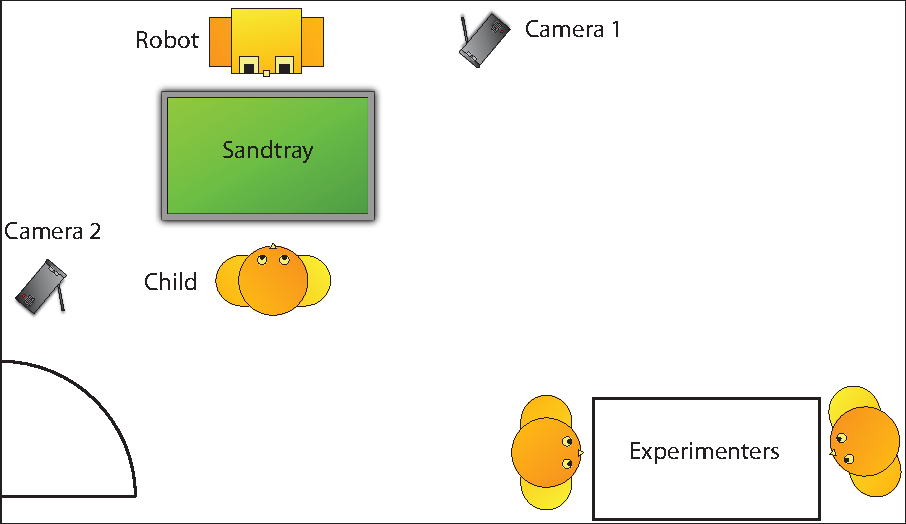
\includegraphics[width=0.7\textwidth]{images/ch6_schematic.pdf}
    \caption{Schematic overview of the mediation device-centred interactions under investigation in this chapter. Two interactants (the child and the robot) face one another over the touchscreen. Two video cameras record the interactants during the studies. The experimenters are also in the room, but out of view of the child. Figure not to scale.}
    \label{fig:ch6-schem}
\end{figure}

\subsection{Alien Sorting Task}\label{sec:ch6-meth-sorttask}
Pilot studies showed that overriding children's prior knowledge in a relatively short (5-10 minute) interaction time is extremely challenging; prior knowledge can play a large part in learning \citep{smith1994misconceptions}. It has been shown that differing knowledge levels lead to different interpretations of a problem \citep{chi1981categorization} and also require substantially different teaching formats to cope with this \citep{kalyuga2008relative}.  To remove these factors, a task with which all children have the same level of knowledge is therefore desirable. As such, the most practical solution is a task that the children have no prior knowledge about. To this end, a novel sorting dataset was created using aliens (as inspired by \citealp{lupyan2007language}).

An online `alien creator' associated with a children's television programme was used to produce aliens of different morphologies and colours. Each alien consisted of six main body parts: a torso, a head, two legs, two arms, wings and a tail. There were three body types which each had different options for the body parts. Approximately 220,000 different combinations could be created. Each body part can then be coloured using the full RGB colour space. From this, a random subset of 96 unique alien images were created. These were split into six training sets and two test sets of equal sizes (12 images per set).

The sorting task required the children to make a binary categorisation on the Sandtray touchscreen. A sorting rule was formulated that was based on one feature: given the wide range of possible features (and indeed combinations of features) that the rule could be based on, it is unlikely that the rule would be discovered by chance in the short period of the interaction. In this case, aliens with yellow legs would be correct if placed in the `purple planet' category; all aliens which did not have yellow legs belonged to the `orange planet' category (Figure~\ref{fig:ch6-alienandcats}). Twelve aliens would be presented to the children in each image set for categorisation and would be split equally between the categories; 6 aliens of each set would belong each category. Children could drag an alien across the screen and release it over the category that they thought it belonged to. The category icon would then change to display either a large green tick, or a large red cross depending on whether the categorisation was correct or not.

\begin{figure}[t!]
    \centering
    \includegraphics[width=0.9\textwidth]{images/ch6_Combined.pdf}
    \caption{From \textit{left} to \textit{right}: (1) the `orange planet' category image, (2) an outline of one of the aliens with shading to differentiate the body parts which can be manipulated (an actual image has not been used due to copyright restrictions), (3) the `purple planet' category image}
    \label{fig:ch6-alienandcats}
\end{figure}

\subsection{Robot Behaviour}\label{sec:ch6-meth-robobehave}
A behaviour for the robot was created by analysing the behaviour of a human tutor (an education professional) when guiding a student unknown to them through a sorting task on the Sandtray, as in \cite{kennedy2013constraining}. The human tutor was told that they would be assisting the child in guided discovery learning and that they could use any technique to guide the child, provided that they did not explicitly state the categorisation rule (as this would then no longer constitute discovery learning). 

Two preparatory sessions were conducted with different children interacting with a human tutor. These underwent video analysis in order to get an objective measure of particular movements and vocalisations made in the interaction by the tutor. The most common verbal phrases, along with the timing and types of screen movements made were used as a basis for the robot behaviour. The result was a script that the robot would follow to introduce itself and the task to the child (full transcript available in Appendix~\ref{app:ch6-robotscript}), along with a guiding behaviour for the discovery learning part of the task. The guided discovery assisting behaviour of the robot consisted of the following elements:

\begin{enumerate}
	\item Verbal feedback specific to the image categorised by the child whenever a categorisation was made.
	\item Advancing the screen library when all of the images in a particular set had been categorised, along with a general hint about the pattern.
	\item If the child did not make a categorisation for 6 seconds, the robot would select an image, move it to the centre of the screen and make a verbal comment to the child about the item. This will be referred to as the robot `highlighting' an image.
	\item A gaze towards the child was also made when making a comment and highlighting a possible move.
\end{enumerate}

Given that these child-responsive robot behaviours are directly inspired by the behaviour of the human teacher, we contend that it therefore demonstrates some key aspects of social behaviour in a tutoring context. The touchscreen provided the robot with information about the visible images, allowing the robot to make comments such as ``why don't you try this one with purple wings?'', or ``pink legs worked in that one''. This was the mechanism by which children were encouraged to think about the properties of the aliens that they were categorising and to lead them towards the correct solution. Of course, it would be straightforward to inform the children of the pattern and then see how well they recall it, but the benefits from guided learning, as outlined in \cite{kuhlthau2007guided, merrill1995tutoring} and the introduction to this chapter, would not be leveraged in this case.

The robot behaviour was structured such that the speech could be blocked depending on its importance and events on screen. The aim was for the robot to provide feedback on every move made by the child, however if the child then categorised images at a very quick rate, the robot speech would not be able to keep up. To solve this, a blocking period of 2 seconds was put in place after each robot vocalisation. In cases where the child was making extremely fast categorisations (approximately one per second), two phrases could follow one another before the blocking period would begin. The speech blocking period could be ignored if the intended speech had been marked as \textit{important} in the code. Speech which was part of the robot script and the general comments made at the end of each library (often key hints for solving the task) were classed as important speech which could ignore the blocking period in order to ensure equality across conditions and interactions. This speech planning strategy ensured that all children experienced the same structure to the interaction, whilst remaining adaptive to individual behaviour.

At the start and end of the interaction, alongside the scripted speech, the robot would make a number of predefined gestures and gaze upwards, towards the child, in a similar way to the human teacher. For the rest of the interaction, the robot would randomly move its head and body to give it a `lifelike' feel. The random gaze was restricted to operate within a rectangular volume roughly directed towards the touchscreen while the child was moving images, as seen in previous human-human and human-robot studies with this task and the touchscreen \citep{baxter2013emergence, kennedy2013constraining}.

The robot behaviour was almost fully autonomous, with input required only to start the interaction and to start the post-test at the appropriate time. Following the protocol for a large number of \acrshort{hri} studies, a Wizard-of-Oz (\acrshort{woz}) experimental technique was adopted to serve this purpose (definitions and descriptions of \acrshort{woz} use in \acrshort{hri} can be found in \citealp{riek2012wizard}). A Wizard was needed simply to click a button to start the interaction once the child was present and to start the post-test once the time limit had been reached for the teaching behaviour (see Section~\ref{sec:ch6-meth-intscen} for more details of this). The Wizard was one of the experimenters located in the room with the child, as described in Section~\ref{sec:ch6-meth-setup}.

\subsection{The Learning Task}\label{sec:ch6-learning-task}
The learning task required children to explore the images presented on-screen and discover, through trial and error, the rule that yellow legged aliens belonged on the purple planet. The robot would assist by making suggestions and providing hints about features to test, as described in Section~\ref{sec:ch6-meth-robobehave}. Without the robot's assistance, the children would only have ticks and crosses displayed on screen for each categorisation as feedback. This would make the task one of reinforcement learning; the screen providing the positive or negative reinforcement on each categorisation. Children do not respond to feedback as effectively as adults and take many more trials to incorporate feedback into their strategy-making \citep{crone2004developmental}.

Additionally, given the balancing of the task, half of the information they see belongs in one planet, and half in the other. With no knowledge of the rule before they start, they are likely to get some categorisations wrong. This can lead to acquisition of erroneous information simply because they have had that thought before, even if negative feedback is provided; the `mere-exposure' effect \citep{begg1985believing, roediger2006power}.

Section~\ref{sec:ch6-meth-sorttask} showed that there are around 220,000 alien body combinations that could be created, with each of the 6 body parts on each alien coloured differently, and each alien of a different size. This presents an overwhelming number of possible features on which to categorise the aliens. If utilised, the hints from the robot substantially reduce this search space, making the solution then possible to reach within the time provided. Given the short interaction time, the complexity of the dataset and the way children learn with just reinforcement feedback, it would be highly unlikely for them to find the correct solution without the help of the robot.

\subsection{Measuring Learning}\label{sec:ch6-measure-learn}
As is commonly applied in \acrshort{hri} studies examining learning, pre- and post-tests (as described in \citealp{dimitrov2003pretest}) were used to measure the learning of the child. The children were given as long as they liked to complete the pre- and post-tests, so that there was no time pressure. The pre- and post-tests were novel from the learning data and from each other. Using two different tests, the images of which were not present in the training data, means that learning is measured on novel data in both pre- and post-test conditions. This eliminates any biasing because of familiarity with the data.

The tests used each consisted of 12 aliens which had to be categorised into either the purple or the orange planet, as per the alien sorting task described in Section~\ref{sec:ch6-meth-sorttask}. Prior to the pre-test, the children had been introduced to the task by the robot; for the full script used here, please refer to Appendix A. The children had been instructed as to the nature of the task - sorting aliens into planets - but had no further indications as to what the categorisation rule may be based on.

The two tests were used in a cross-testing strategy; test `A' was administered to half of the children as a pre-test, who then took test `B' as a post-test. The other half of the children took the tests the other way around. The test used for the pre- and post-test was swapped between each interaction, i.e., Child 1 would take Test A as a pre-test and Test B as a post-test, then Child 2 would take Test B as a pre-test and Test A as a post-test. Given the novelty of the material to be learned, this strategy allows analysis to determine whether learning gains can be attributed to differences in difficulty between tests, should any such differences unintentionally arise due to unknown aggravating factors. The category positions would also switch between tests (and indeed in the training sets) to avoid any conditioning to spatial locations.

\subsection{Interaction Scenario} \label{sec:ch6-meth-intscen}
The interaction is largely unstructured and the children are free to work at their own pace. The robot provided verbal feedback on moves that the child made, and would suggest a move to the child if 6 seconds passed without the child making a categorisation. This allowed the child to involve the robot as much, or as little, as they desired based on how long they waited between moves.

The following interaction scenario was created by combining the human teacher model with the lessons learnt from earlier work:
\begin{enumerate}
	\item The robot and touchscreen are introduced to the child by the experimenter. The child is told that they are free to stop at any time, or ask questions of the experimenters.
	\item The robot introduces itself to the child and outlines the task to be completed.
	\item The child completes the pre-test on the Sandtray.
	\item The robot provides a `clue' for the child and begins the guided discovery behaviour while the child categorises further image libraries.
	\item After 5 minutes, the robot brings the guided session to a close and asks the child to complete the post-test, again on-screen.
	\item Once the child has completed the post-test, the robot thanks the child and says goodbye.
	\item The child is debriefed by the experimenters.
\end{enumerate}

Due to the unstructured nature of the task, strict time limits could not be set for the interaction. As the guided discovery behaviour of the robot was the main variable being measured, an effort was made to keep this a consistent length of time. The target length of time was set at 5 minutes, as this was estimated to make the total interaction around 7-10 minutes long; an appropriate length as identified in the pilot studies. The Wizard would have a button to click once the child was nearing the end of an image library in the fourth minute of the teaching behaviour. This would then trigger the post-test script at the end of the current library.

The average length of an interaction was \textit{M}=533 seconds, \textit{SD}=58s. This was measured from the moment the child entered the experiment room, until the moment that they left. The average length of the learning phase was \textit{M}=308s, \textit{SD}=45s.

\subsection{Video Data} \label{sec:ch6-meth-intdata}
All 28 videos were coded by one coder, with validation from a second coder. It is not practical to second code all of the video due to the amount of time this takes. Therefore, a proportion (18\%) of the videos were second coded to validate the first coder, following the example set by \cite{moshkina2014social}, \cite{nalin2012children} and \cite{stanton2008robotic}. The videos for second coding were randomly selected from groups which ensured proportional representation between experimental conditions, experimental days and genders. The overall inter-coder agreement level, Cohen's kappa, across all tracks was an average of 0.78, which indicates \textit{substantial} agreement \citep{landis1977measurement}. The coding scheme used was as objective as possible, based solely on overt child or robot behaviour and can be seen below. Table~\ref{tab:ch6-coderagree} shows the agreement for the tracks which will be used for analysis in Section~\ref{sec:ch6-results-inter}.

\begin{itemize}
	\itemsep-0.2em
	\item Interaction stage
	\item Child gaze
	\item Child gestures
	\item Child vocalisations
	\item Robot gaze
	\item Robot gestures
	\item Robot vocalisations
\end{itemize}

\begin{table}[t!]
	\centering
	\renewcommand{\arraystretch}{1.2} 
	\begin{tabular}{@{}p{4.5cm}p{3cm}@{}}
	\toprule
	\textbf{Track} 			& \textbf{Cohen's Kappa} \\ \midrule
	Overall agreement 	& 0.78\\
	Child gaze 				& 0.89\\
	Child gestures 			& 0.84\\
	Robot gaze 				& 0.63\\
	Robot gestures 		& 0.76\\ \bottomrule
	\end{tabular}
	\caption{Inter-coder agreement by track coded.}
	\label{tab:ch6-coderagree}
\end{table}

%%%%%%%%%%%%%%%%%%%%%%%%%%%%%%%%%%%%%%%%%%%%%%%%%%%%%
\section{Learning Results} \label{sec:ch6-embodiment-results}
Twenty-six pairs of pre- and post-tests were logged during the interactions for analysis of learning. Two different tests were used as described in Section~\ref{sec:ch6-measure-learn}, named \textit{Test A} and \textit{Test B} for ease of discussion here.

When considering the population as a whole, a significant learning effect is found between the pre- and post-tests. Two groups are compared with paired values on a continuous measure, distributions did not significantly deviate from normality (Kolmogorov-Smirnov test; $\textit{p}>.05$). As such, a paired samples \textit{t}-test is used. A paired \textit{t}-test reveals that the post-test score (\textit{M}=9.12, 95\% CI [8.13,10.10]) was significantly higher than the pre-test score (\textit{M}=7.08, 95\% CI [6.34,7.82]); \textit{t}(25)=3.016, \textit{p}=.006. However, when the learning effect is examined in more detail, a more complex story is revealed. Children who completed Test A as a pre-test and Test B as a post-test did not exhibit significant learning, whereas for the reverse (Test B to A), extremely significant learning was found (Table~\ref{tab:ch6-learnttests}). This complication is due to the comparative `difficulty' of the tests given no knowledge of the data and biases which are present, to be discussed in Section~\ref{sec:ch6-biasing}.

\afterpage{%
	\begin{landscape}
		\begin{table}[t!]
			\centering
			\renewcommand{\arraystretch}{1.2} 
			\begin{tabular}{@{}p{2.5cm}p{2.5cm}p{3.8cm}p{4.7cm}p{4.7cm}p{1.5cm}p{1.9cm}@{}}
			\toprule
			\textbf{Condition A} & \textbf{Condition B} & \textbf{\textit{t}-test used} & \textbf{Condition A \textit{M} (\textit{n}, 95\% CI)} & \textbf{Condition B \textit{M} (\textit{n}, 95\% CI)} & \textbf{\textit{p} value} & \textbf{\textit{t} (\textit{df})} \\ \midrule
			Pre-test A & Post-test B 		& Two tailed, paired 		& 7.93 (14, [6.88,8.98]) 	& 8.43 (14, [6.74,10.12]) 	& .627 & \textit{t}(13)=0.498 \\
			Pre-test B & Post-test A 		& Two tailed, paired 		& 6.08 (12, [5.25,6.92]) 	& 9.92 (12, [9.00,10.83]) 	& $<$.001* & \textit{t}(11)=6.823 \\
			Virtual gain & Real gain 	& Two tailed, unpaired & 2.42 (12, [0.65,4.18]) 	& 1.71 (14, [-0.60,4.03]) 	& .614 & \textit{t}(24)=0.510 \\
			Pre-test A 	& Post-test A 	& Two tailed, unpaired & 7.93 (14, [6.88,8.98]) 	& 9.92 (12, [9.00,10.83]) 	& .005* & \textit{t}(24)=3.051 \\
			Pre-test B 	& Post-test B 	& Two tailed, unpaired & 6.08 (12, [5.25,6.92]) 	& 8.43 (14, [6.74,10.12]) 	& .017* & \textit{t}(24)=2.558 \\ \bottomrule
			\end{tabular}
			\caption{Learning effect \textit{t}-test results, comparing many different variables. `Gain' refers to the increase in score between pre- and post-tests. The maximum score for all conditions is 12. * indicates a significant \textit{p} value at the .05 level. All distributions do not significantly deviate from normality (Kolmogorov-Smirnov test; $\textit{p}>.05$). For unpaired tests, observations are independent. All measures are continuous.}
			\label{tab:ch6-learnttests}
		\end{table}
	\end{landscape}
}

When considering the calculated bias values in the context of the tests, if the biases are followed, then a child would get 9 out of 12 correct on Test A and 7 out of 12 correct on Test B. This is reflected in the actual pre-test scores acquired: children scored average of 7.93 (95\% CI [6.88,8.98]) for Test A and an average of 6.08 (95\% CI [5.25,6.92]) for Test B. Additionally, this explains why learning effects measured from Test A to Test B may be hidden, and from Test B to Test A, may be amplified. Whilst the `gain', the improvement in the score from pre- to post-test, is higher on average for the virtual robot than the real robot, this is not statistically significant (Table~\ref{tab:ch6-learnttests}).

\subsection{Learning Bias} \label{sec:ch6-biasing}
Significant learning effects are observed when Test B was used as the pre-test, but the same was not found for Test A as the pre-test. To explore why this occurred, every pre-test image categorisation was analysed. It became apparent that whilst the datasets used had been carefully designed to be novel and prevent children having preconceptions, they were not immune to biasing effects. Clear patterns emerged in the way that the children categorised the aliens in the pre-test; the point at which they had no knowledge of the dataset material. 

Upon further investigation of the literature it was discovered that children start to use colour as a predictor of category membership from an early age, as shown in \cite{macario1991young}. Combining this indication from the literature and examining the consistently incorrectly categorised aliens, the following hypothesis was formulated about the bias of colour in the dataset:
\begin{itemize}
	\item Given no knowledge of the dataset, the greater the proportion of purple on an alien, the more likely it is to be categorised on the purple planet.
	\item Similarly, the same is true for orange on an alien and the orange planet.
\end{itemize}

Children were consistent at applying this bias and it was concluded that a bias-free dataset would be almost impossible to create. If the bias could be quantified then learning effects in spite of the bias, or on minimally biased images, could be evaluated. The equation shown in~\ref{eq:ch6-bias} was formulated as a measure of bias.
\begin{equation}\label{eq:ch6-bias}
	bias = \%P - \%O
\end{equation}

Where:
\begin{itemize}
	\item $\%P$ = the percentage of pixels perceived to be purple out of the total number of coloured pixels in the image.
	\item $\%O$ = the same as the above for orange pixels.
\end{itemize}

This results in a bias value between -1 and 1. A value of 0 represents no bias, a negative value is a bias towards the orange planet and a positive value is a bias towards the purple planet. The greater the magnitude of the number, the greater the bias effect. This equation assumes no bias when neither purple or orange are present in an image and takes into account the relative balance between purple and orange in an image; if they are equal then they will cancel each other out.

In order to evaluate the effect of the colour bias, a series of paper-based tests were given to a different group of children. Three different tests were used: two were the test sets from the main study and a third test was created to investigate aspects of the biasing hypothesis. Each test had twelve images of aliens in a vertical line in the centre, with the planets aligned to the right and left edges of the page. The side on which the purple and orange planets were placed was varied between the tests. A total of 54 tests were completed; 18 of each different test. 24 males and 30 females completed the tests, the children were aged 7 or 8 years old (\textit{M}=7.2, \textit{SD}=0.54).

The percentage of pixels which were purple and orange was counted for each of the 36 images used across the three tests. These values were then inserted into Equation~\ref{eq:ch6-bias} to provide a bias value for each of the images. Correlation between the calculated bias values and the actual percentage of children which categorised the image as purple or orange was then measured. Pearson's product-moment correlation coefficient shows a very strong correlation of \textit{r}(34)=0.761 (\textit{p}$<$.001) between bias value and percentage categorised as purple, and \textit{r}(34)=-0.761 (\textit{p}$<$.001) between bias value and percentage categorised as orange. The correlations are the inverse of one another due to the inverse relationship between the percentage categorised as purple and orange.

As the bias value holds a strong correlation to the actual child behaviour, this can be used to divide the test sets into groups based on their relative biasing. This is useful because it allows learning effects to be considered in the context of the bias. There are some clear clusters and a division of 0.2 and -0.2 was used to split the groups (Figure~\ref{fig:ch6-biasscatter}):
\begin{itemize}
	\item $bias >  0.2 = 9$ images biased towards purple
	\item $-0.2 < bias < 0.2 = 9$ minimally biased images
	\item $bias < -0.2 = 6$ images biased towards orange
\end{itemize}

\subsection{Accounting for Bias} \label{sec:ch6-results-bias}
Table~\ref{tab:ch6-learnttests} shows a significant increase between those children taking pre-test A and those taking post-test A \textit{and} a significant increase between pre-test B and post-test B. This cross-comparison could be used to make an argument for overall significance of learning effects in spite of differences between the tests. However, it is more convincing to consider learning effects taking into account the known biases. The children's tests will now be evaluated in the context of the bias groups as laid out in Section~\ref{sec:ch6-biasing}. If learning is indeed present, the following hypotheses would be true:
\begin{itemize}
	\item [\textbf{H$_{0}$:}] Images with minimal biasing will be categorised more correctly in the post-test than the pre-test.
	\item [\textbf{H$_{1}$:}] Images with large biasing towards a correct category remain unchanged.
	\item [\textbf{H$_{2}$:}] The bias of images with large biasing towards an incorrect category will be reversed.
\end{itemize}

\begin{figure}[t!]
    \centering
    \includegraphics[width=0.7\textwidth]{images/ch6_BiasScatter.pdf}
    \caption{Calculated bias value for each of the images used in the experimental pre- and post-tests using Equation~\ref{eq:ch6-bias}.}
    \label{fig:ch6-biasscatter}
\end{figure}

H$_{1}$ and H$_{2}$ make it necessary to divide the images with a large bias into two smaller groups: those where the bias leads to a correct categorisation and those where it leads to an incorrect categorisation. In regard to H$_{1}$, the number of correct categorisations will not change if learning is present, but it is hoped that the reasoning behind the categorisation changes from bias-influenced to knowledge-based. Unfortunately, it is not possible to measure the reasoning behind a classification given the current task.

In order to test these hypotheses, the percentage of correctly categorised images in the pre- and post-tests were grouped together based on the strength and direction of the bias. Four images are biased towards an incorrect categorisation, 11 images are biased towards correct categorisation and 9 images are minimally biased. Each image is categorised between 12 and 14 times.

The increase for minimally biased images is not significant, which does not support hypothesis H$_{0}$. The increase for images with a large bias towards a correct classification is also not significant, meaning that H$_{1}$ is supported. H$_{2}$ is also supported; a significant effect is found between pre- and post-test scores for those images biased towards an incorrect categorisation (Figure~\ref{fig:ch6-combinedbias}, Table~\ref{tab:ch6-biasgroups}). The bias groupings were considered across the two embodiment conditions, but no significant differences were found.

\begin{table}[t!]
	\centering
	\renewcommand{\arraystretch}{1.2} 
	\begin{tabular}{@{}p{3cm}p{3.2cm}p{3.2cm}p{1.5cm}p{1.9cm}@{}}
	\toprule
	\textbf{Bias group} & \textbf{Pre-test (95\% CI)} & \textbf{Post-test (95\% CI)} & \textbf{\textit{p} value} & \textbf{U value} \\ \midrule
	Minimal 			& 62\% [52,72] 	& 72\% [61,82] 	& .202		& 70.5 \\
	Bias to correct 	& 72\% [64,80]	& 79\% [71,87] 	& .197		& 70.5 \\
	Bias to incorrect 	& 9\% [1,17]	& 77\% [62,92] 	& $<$.001* 	& 12.5 \\ \bottomrule
	\end{tabular}
	\caption{Learning effect Mann-Whitney U test results grouped by bias. All observations are independent, but some distributions deviate significantly from normality (Kolmogorov-Smirnov test; $\textit{p}<.05$), making the U test more efficient than \textit{t}-tests. Average percent correct is shown for both pre- and post-tests. * indicates a significant \textit{p} value at the .05 level.}
	\label{tab:ch6-biasgroups}
\end{table}

\begin{figure}[t!]
    \centering
    \includegraphics[width=0.8\textwidth]{images/ch6_BiasLearning.pdf}
    \caption{Pre-test and post-test percentage of correct answers for images, grouped by bias type and direction. \textit{Error bars} show the 95\% Confidence Interval.}
    \label{fig:ch6-combinedbias}
\end{figure}

%%%%%%%%%%%%%%%%%%%%%%%%%%%%%%%%%%%%%%%%%%%%%%%%%%%%
\section{Behaviour and Embodiment Results} \label{sec:ch6-results-inter}
This section will analyse the relationship between the behaviour of the children, behaviour of the robot and the embodiment condition. Previous work suggests that embodiment will have an effect on the children's behaviour, as discussed in the introduction to this chapter and Chapter~\ref{chap:background}. This analysis is necessary in order to explore Hypotheses 2 and 3. This section will first analyse the children's compliance with the robot's suggestions, which relates to Hypothesis 2. The two subsections after will consider different aspects of the gaze behaviour of the child, which both relate to Hypothesis 3.

\subsection{Compliance}
The children clearly complied with the robot's suggestions for moves, as the percentages of responses below show (Figure~\ref{fig:ch6-piechart}). Even when the children were in the process of completing a move themselves, they were significantly more likely to stop their current move and follow the robot's suggestion than not \citep{kennedy2014children}.

\begin{itemize}
	\item 87\% of the moves which the robot suggested were taken immediately by the children
	\item 4\% were taken after the child had finished any move that they had already begun
	\item 4\% of the suggested moves were ignored by the children
	\item 5\% were occluded in the video analysis
\end{itemize}

\begin{figure}[t!]
    \centering
    \includegraphics[width=0.6\textwidth]{images/ch6_PieChart.pdf}
    \caption{Child responses to robot suggestions to make a move. Children clearly comply with the robot's requests.}
    \label{fig:ch6-piechart}
\end{figure}

Two groups were used with independence of observations, and a continuous measure. Distributions did not significantly deviate from normality (Kolmogorov-Smirnov test; $\textit{p}>.05$) and had homogeneity of variances (Levene's test; $\textit{p}>.05$). For this reason, two-tailed independent samples \textit{t}-tests are used to analyse the results. When performing this test, there were no significant differences between the two embodiment conditions for the number of moves taken immediately (\textit{t}(26)=1.568, \textit{p}=.129), although the real robot had a slightly higher average (\textit{M}=89.5\%, 95\% CI [77.7,101.3]) compared to the virtual robot (\textit{M}=77.7\%, 95\% CI [66.9,88.6]). No significant correlation was found between the number of suggested moves by the robot and the improvement in score between pre- and post-tests; Pearson's \textit{r}(24)=--0.137, \textit{p}=.507.

The high level of compliance with the robot's suggestions provides an indication that the children were engaged with the robot as well as the task throughout the interaction. This provides partial support for Hypothesis 2, although further evidence is required to fully support this hypothesis.

\subsection{Gaze and Embodiment}
When considering the full length of the interaction, there were a number of significant findings in the differences between the children's gaze and touchscreen gestures towards the real and virtual robot. Two groups were used with independence of observations, and a continuous measure. Distributions did not significantly deviate from normality (Kolmogorov-Smirnov test; $\textit{p}>.05$) and had homogeneity of variances (Levene's test; $\textit{p}>.05$). For this reason, two-tailed independent samples \textit{t}-tests are used to analyse the results. Children interacting with the real robot (\textit{M}=5.19, 95\% CI [4.48,5.91]) make significantly more gazes towards the robot per minute than those in the virtual robot condition (\textit{M}=4.13, 95\% CI [4.48,5.91]), \textit{t}(26)=2.296, \textit{p}=.030. The length of each individual gaze is similar between conditions, so those in the real robot condition (\textit{M}=9.40, 95\% CI [8.36,10.44]) spend significantly more seconds per minute of interaction gazing towards the robot than those interacting with the virtual robot (\textit{M}=7.53, 95\% CI [6.37,8.70]), \textit{t}(26)=2.586, \textit{p}=.016. This result confirms findings from \cite{looije2012help} in a new context, and also supports Hypothesis 1.

Repeated measures ANOVAs are used to compare the effect of interaction time on the childrens' gaze towards the robot. Greenhouse-Geisser correction is applied due to violation of the assumption of sphericity (Mauchly's test $\textit{p}<.05$). For the \textit{virtual} robot condition, there is a significant effect of interaction segment on child gaze towards the robot at the \textit{p}$<$.05 level for the three segments [\textit{F}(1.10,13.15)=7.504, \textit{p}=.015]. However, post-hoc pairwise tests with Bonferroni correction find no significant differences between the individual stages (all \textit{p}$>$.05). For the \textit{real} robot, there was a significant effect of interaction segment on child gaze towards the robot at the \textit{p}$<$.05 level for the three conditions [\textit{F}(1.16,16.23)=7.089, \textit{p}=.014]. Post-hoc comparisons with Bonferroni correction indicated that the mean score for the first segment (\textit{M}=6.64, 95\% CI [4.83,8.44]) was significantly different to the second segment (\textit{M}=4.26, 95\% CI [3.67,4.85]) and to the third (\textit{M}=4.42, 95\% CI [3.59,5.25]); \textit{p}=.013 and \textit{p}=.023 respectively. The second and third segments had no significant difference, \textit{p}=1. This means that the gaze significantly dropped from the first to the second interaction segment for the real robot and then remained at roughly the same level as the second for the third. For the virtual robot, the same pattern is seen, but the changes are not as large. The comparison of these two curves can be seen in Figure~\ref{fig:ch6-gazemainint}.

\begin{figure}[t!]
    \centering
    \includegraphics[width=0.7\textwidth]{images/ch6_GazeBySectionVvsR.pdf}
    \caption{Seconds per minute that the child spends gazing towards the robot, split by learning phase third, comparing embodiment conditions. \textit{Error bars} show 95\% Confidence Interval.}
    \label{fig:ch6-gazemainint}
\end{figure}

It is suggested that the drop in gaze for the virtual robot is smaller than for the real robot because the starting level is lower than that of the real robot. Because of this lower starting point there is less of a reduction in gaze which is possible (a floor effect), whereas the relatively high starting point for the real robot gaze level allows for a greater drop. In the third segment, the gaze remains and roughly the same level as in the second segment for both conditions. This is an indication that once the children become accustomed to the social behaviour of the robot their interest in the robot drops off, reflected by their reduced gaze towards it \citep{baxter2014tracking}. When novel social behaviour is re-introduced for the post-test, the engagement level then raises again, in agreement with \cite{szafir2012pay}.

\subsection{Gaze and Robot Behaviour} \label{sec:ch6-results-segments}
Considering the interaction as a whole reveals a number of interesting results, but considering the interaction in terms of its component parts, as laid out in Section~\ref{sec:ch6-meth-intscen}, allows a more thorough analysis and the exploration of behaviour over time. This has previously been suggested for use as a ``proxy for engagement in the interaction or for the human's attribution of social agency to the robot'' \citep{baxter2014tracking}. Gaze can be converted into seconds per minute values in order to normalise between individuals and allow for direct comparison.

The amount of gaze towards the robot varies a lot between the different segments (Figure~\ref{fig:ch6-gazesegments}). When the robot is directly addressing the child, the child gazes more towards the robot than when the robot is not addressing the child at all; a good example is the difference between when the robot is providing instructions and when the child is completing the pre-test. The gaze for the learning phase appears to be quite low in comparison to some of the other sections; whilst it is, this does not mean that the child is not paying attention to the robot. It is possible for the child to observe the robot's actions on screen and to get feedback from the screen, whilst also listening to the robot; this could explain the relatively low level of gaze towards the robot throughout this phase of the interaction. Another notable difference is seen between the gaze towards the robot during the pre- and post-tests; this will be discussed further in Section~\ref{sec:ch6-disc-social}.

\begin{figure}[t!]
    \centering
    \includegraphics[width=0.9\textwidth]{images/ch6_RvsVFull.pdf}
    \caption{Seconds per minute that the child spends gazing towards the real and virtual robots, split by interaction segment. \textit{Error bars} show 95\% Confidence Interval.}
    \label{fig:ch6-gazesegments}
\end{figure}

Of particular interest is the behaviour of the child during the main learning phase. As the stages are 3 related measures, a within-subjects repeated measures ANOVA was conducted to compare the effect of interaction time on the child's gaze towards the robot (both conditions combined). Greenhouse-Geisser correction is applied due to violation of the assumption of sphericity (Mauchly's test $\textit{p}<.05$). The learning phase was split into thirds for comparison \citep{baxter2014tracking}. There was a significant effect of interaction segment on child gaze towards the robot at the \textit{p}$<$.05 level for the three thirds [\textit{F}(1.14,30.87)=13.920, \textit{p}$<$.001]. Post-hoc comparisons with Bonferroni correction indicate that the mean score for the first segment (\textit{M}=5.63, 95\% CI [4.48,6.79]) was significantly different to the second segment (\textit{M}=3.56, 95\% CI [2.84,4.28]) and the third segment (\textit{M}=3.73, 95\% CI [2.99,4.47]), with \textit{p}=.004 and \textit{p}.008 respectively. No significant difference was found between the second and third segments, \textit{p}=1. Therefore, children look at the robot significantly more in the first third of the learning phase, before dropping for the rest of the interaction.

%%%%%%%%%%%%%%%%%%%%%%%%%%%%%%%%%%%%%%%%%%%%%%%%%%%%%
\section{Discussion} \label{sec:ch6-embodiment-discussion}
This section will discuss the overall learning significance in relation to the task and the robot, the lack of learning differences between the real and virtual robot conditions, and the significant behavioural differences in the response of children to the real and virtual robots. Addressing these points allows conclusions to be made in response to the hypotheses laid out in Section~\ref{sec:ch6-hypoth}.

\subsection{Embodiment and Learning}\label{sec:ch6-disc-learning}
No significant differences were found in learning between those children who interacted with the real robot and those who interacted with the virtual robot. Other studies have found significant differences between different robot embodiments, for example \cite{huang2013modeling, leyzberg2012physical}. In this case these effects were not found; thereby not supporting Hypothesis 4. However, this is in line with some work, for example \cite{hasegawa2010role}. Given the context of the interaction, it is suggested that the robot's behaviour had a greater impact on learning than its embodiment.

The length of the interactions may have caused the lack of difference between the embodiment conditions. The learning phase of the interaction was an average of 309s; just over 5 minutes. This is a very short amount of time for learning, meaning that the task had to be simple. Additionally, the social behaviour of the robot was limited. The scripted elements of the interaction were relatively rich, but the main learning phase was repetitive and it indeed appears that the children lost interest in the robot as they became aware that the robot was not socially responsive (Section~\ref{sec:ch6-results-segments}). If the robot could exhibit richer social behaviours during the learning phase then it may be that a greater difference between the children's reactions towards the robot would be observed, which may improve the learning outcome.

The learning differences between the real and virtual robots may also have been influenced by the novelty effect. Not only were the children facing a novel robot, in whichever form that may take, but also a large touchscreen. It is likely that even if there are differences in how children would respond to either of the robot embodiment conditions, they would be excited by the novel technology in either condition and therefore more likely to give the task their maximum attention, reducing any potential for difference between conditions in task performance.

One way to disentangle the novelty effect would be to carry out the experiment over a longer length of time so that the effect wears off. However, this would certainly require a change in the complexity of the task to prevent it quickly becoming boring for the children. Although a study of this nature could be interesting, it may not yet be as useful as it could be. It would be beneficial to establish the importance of a more socially responsive behaviour for the robot, and then consider the impact of this over time.

With a larger sample size it is possible that learning differences may then become more pronounced and could also be generalised. The difficulty would then be in recruiting enough subjects of the correct age, particularly given the challenges in recruiting subjects and running studies outside of the lab, as highlighted in \cite{ros2011child} and \cite{walters2005practical}.

\subsection{Social Behaviour and Embodiment}\label{sec:ch6-disc-social}
When considering the social behaviour exhibited by the children between the two conditions, the main difference was in the amount of time the children spent looking at the real robot; they look at the real robot significantly more than the virtual robot. An increased amount of gaze towards a real robot when compared to a virtual one has been seen in other studies as well, for example \cite{looije2012help}, and the increased mobility of the real robot has been suggested as an explanation, as in \cite{breazeal2004social}.

The ability of the real robot to enter into the child's field of vision whilst they are looking at the touchscreen is a great advantage. This can be used as a technique to direct the child's attention during the task, or to make sure that the child is paying attention \citep{szafir2012pay}. This could be particularly useful in a more complex task where the robot's input is more tightly coupled to the learning outcome.

Because of the differences in embodiment and the subsequent lack of depth information when looking at the virtual robot, the virtual robot (\textit{M}=15.4, 95\% CI [12.8,17.9]) appears to gaze at the child significantly more than the real robot (\textit{M}=10.5, 95\% CI [8.2,12.9]) when normalised to s/min, \textit{t}(26)=3.029, \textit{p}=.005. It is surprising that this does not cause the child to look at the virtual robot more often in order to reciprocate this gaze. The real robot attracts significantly more gaze from the child than the virtual robot and if the robot behaviour were to be more varied then it is possible that the heightened levels of gaze seen at the start of the learning phase could be maintained. This could be used to argue that the real robot has the potential to be more socially engaging than the virtual robot and that this may lead to increased task performance in the future. 

The mediator has a large effect on the social interaction which takes place; the mediator attracts the majority of the gaze from the child and in it's current form, the children can get all the information they need to play purely from the screen once the task has started. Something which may reduce the large disparity between gaze towards the robot and the touchscreen could be to remove any feedback elements from the touchscreen; if the feedback on the screen were to be removed, then the robot would be the child's only source of feedback, which may facilitate social engagement. An increased reliance on the robot for feedback could lead to more engagement with the robot from the child, which could improve learning gains.

Additionally, once the child understands the concept of the task, the robot's input is not necessary for completing the task presented here because of the mediator. The children can choose to exclude the robot from parts of the learning phase by taking moves quickly and preventing the robot from suggesting a move. If the coupling between the task and the robot were tighter, it is likely that the behaviour of the robot would have a greater impact on the outcome of the task. From this perspective, the impact may also be more consistent, as the robot involvement would likely be more consistent as well, as opposed to the current setup where the robot input varies depending on how the child behaves. It should be noted that it is not being suggested that this consistency would result in a higher average performance increase; the hypothesis would remain that a more adaptive robot would result in greater child performance.

The results show that the children spend more time looking at the real robot than the virtual robot. It is likely that if the task was more spatially orientated, or required joint reference, the real robot would hold an advantage. In the task used, when the robot suggested a move, it was clear on the touchscreen which image the robot was suggesting, so the gaze of the robot was not needed to identify the object of reference. It may be that if the touchscreen did not make it clear which of the images the robot was pointing to, then the increased gaze towards the real robot may play a more important role in the learning outcome.

The amount of time per minute that the children gaze towards the robot during the pre- and post-tests has previously been highlighted as an interesting difference to discuss. Figure~\ref{fig:ch6-gazesegments} suggests that there would be a significant difference between the amount of time the children spend looking towards the robot during the two testing phases. This is due to the inclusion of the post-test instructions from the robot to the child in the post-test segment. When splitting out this instructional phase, there is very little difference between the gaze towards the robot during the tests. During the pre-test, the children spend an average of \textit{M}=1.0 seconds per minute (\textit{s/m}) gazing towards the robot (95\% CI [0.5,1.5]); this rises very slightly to \textit{M}=1.3 s/m (95\% CI [0.8,1.8]) during the post-test. The post-test gaze towards robot value had been inflated by the inclusion of the instructions in this phase. Whilst the instructions are being given by the robot, the child spends \textit{M}=25.0 s/m (95\% CI [21.1,28.8]) gazing towards the robot. This is almost half of the time and further supports the point made in Section~\ref{sec:ch6-results-segments} suggesting that the children gaze more towards the robot when it is directly addressing them and exhibiting novel behaviour.

\cite{schermerhorn2011disentangling} have demonstrated the complex interactions which occur between embodiment and other elements of robot behaviour. Whilst the analysis of an integrated system is always desirable, we would suggest that varying just one of the dimensions at a time affords the ability to establish a hierarchy between factors which are hypothesised to have an impact on the results and also to make direct attributions between variables and outcomes.

In a similar way, \cite{huang2013modeling} adopt a multivariate analysis approach to study the impact of a specific behavioural variable, in this case gesture, on knowledge recall. This attractive approach affords the ability to study several variables whilst keeping subject numbers low; often a great challenge for \acrshort{hri} research. However, when dealing with social behaviour, it remains to be seen whether these specific sub-behaviours being varied can be statistically extracted from a more complex behaviour and then successfully implemented into a new `optimised' model.

\subsection{Task Characteristics}\label{sec:ch6-disc-task}
The task that the children completed will have had a large effect on the learning which took place. The task is simple so that it is possible to be learnt within the short interaction time. As such, there is a very limited gradient in terms of the learning which can take place; children either figure out the pattern and do very well on the post-test, or they don't and they continue to sort the images according to the colour biases identified in Section~\ref{sec:ch6-biasing}. This means that subtle differences in learning are unlikely; the learning is often binary, which limits the variability between the post-test scores and therefore between conditions. A task which has a greater gradient of learning to measure on has a much greater resolution of measurement and can therefore provide more variability to make comparisons where subtle differences can be more pronounced. Equally, learning could easily be assessed over the full course of the interaction, rather than in just a pre- and post-test; this type of continual assessment is supported in educational literature \citep{guskey2003classroom, myers2007assessing}.

Furthermore, the unit of measure for learning and how learning is defined is important. Completion time of a puzzle has been used, as in \cite{leyzberg2014personalizing}. Whilst time provides a good resolution of learning steps, it is possibly too closely related to motivation, rather than knowledge gain (although there is an undeniable connection between the two) in the context of the task used for the experiment in this paper. Evaluation of skill over the course of the interaction, rather than just in a pre- and post-test setup, may provide more insight into the learning process.

The position of the robot around the mediator may also impact upon the learning outcome. The position of people around a surface has been studied elsewhere and correlations between seating positions and interaction styles have been made, e.g., \cite{scott2004territoriality, tang2006collaborative}. In this case it is proposed that the seating position has not made a significant impact as the studies showing differences have been human-human and have been ambiguous in the way that the interaction partners have been presented to one another. In this experiment, the children were expecting to play a game with a robot which would be there to help them, so competitive behaviours seen elsewhere when interactants face each other are probably overridden by the context here. This is reinforced by the teacher and student roles assumed by the robot and the child.

The task used in this study was designed so that it would be completely novel to the children. The aim was to prevent preconceptions from influencing the learning taking place, as inspired by \cite{lupyan2007language}. However, a side effect of this was an introduction of a colour bias which complicated the results. Additionally, the development of an entirely novel task in this manner removes a lot of the context from the learning. It is thought that context has a great impact on learning and transfer of knowledge \citep{tessmer1997role}. It is possible that the removal of a real-world context in the learning task inhibited the amount that children could learn, possibly contributing to the lack of learning difference between conditions.

The biases present in the dataset used highlight a trade-off between development of a novel task and the introduction of bias. A novel task was desirable here so that learning could easily be measured independently of preconceptions. However, in creating a novel task, biases were inadvertently introduced. For future work it is important that any novel dataset created is tested and validated to remove, or at least balance, any possible bias. Moreover, work in subsequent chapters will instead move away from the use of a novel task due to the complications that this introduces, and the lack of context surrounding the learning. Instead, a task which children could learn from in an interaction that more closely follows their academic curriculum, whilst not overlapping and confounding the measurement of learning is used.

\subsection{Nonverbal Immediacy}\label{sec:ch6-disc-nvi}
The \gls{nonverbalimm} ratings of the robot behaviour provide a further perspective on the learning results that were found in this study. 37 ratings of the real robot, and 35 of the virtual were acquired (for demographic details please see Appendix~\ref{app:crowdsourced}). The real robot received an average \gls{nonverbalimm} score of \textit{M}=51.9 (95\% CI [50.5,53.3]), with the virtual \textit{M}=50.2 (95\% CI [48.5,51.9]). These scores are not found to be significantly different when using an independent samples, two-tailed \textit{t}-test; \textit{t}(70)=1.517, \textit{p}=.134.

The \gls{nonverbalimm} metric considers overt social cues and provides validation that the social behaviour between the conditions could be perceived in the same manner despite the differences in embodiment (and therefore possible issues with identifying gaze direction in the virtual condition). Prior work has found that embodiment can make a large difference to task outcomes \citep{bainbridge2008effect, leyzberg2014personalizing}. The non-significant difference between the \gls{nonverbalimm} scores of the conditions supports the suggestion that the robot behaviour is largely responsible for the learning outcome here, rather than the embodiment. This may have been due to task characteristics or novelty, as previously discussed, or possibly due to age. Previous studies that find differences due to embodiment largely deal with adults rather than children. It may be that embodiment effects are not so pronounced with children, however, further evidence would be required to confirm this suggestion.

\subsection{Sample Size}\label{sec:ch6-disc-sample}
The sample size used in this chapter is 28 after exclusions. When split across 2 conditions, this is half of the sample size per condition compared to those from the previous chapter (28 per condition). Even if no exclusions had taken place, there would still be fewer subjects in the study here when compared to the previous chapter. This has implications in terms of the confidence one can have in the results found here. Children are known to be highly variable in their performance in tasks \citep{siegler2007cognitive}, and for this reason, to make strong conclusions from a study involving children, a larger sample size is often desired.

However, a larger sample size does not come without other considerations. Throughout this thesis, children are recruited through visits to their schools. It is often the case that attitudes towards technology vary by teacher and the teacher's willingness to engage with technology will influence the attitudes of children towards the technology \citep{sariccoban2013pre,teo2006attitudes}. Teacher attitudes are in turn influenced by training \citep{teo2008pre}, and the school ethos towards technology use \citep{sipila2010impact}. For this reason, it is preferable to conduct experiments with a single year group (or class) at a school. This maximises the chance of having children with similar attitudes towards technology, and also offers the possibility to balance for cognitive ability and prior knowledge.

The year group used in Chapter~\ref{chap:validation} was large, whereas the one in this chapter is more typical, hence the drop in sample size. Given the novelty of the robot technology, and the impact that the teacher can have on how children perceive their interaction with the robot \citep{baxter2015wider}, using a single class or year group can provide tighter experimental control despite lower subject numbers. If children from more than one school were to be used, then it is suggested that several schools should be used instead and subject numbers would need to be greatly increased to average out interaction effects introduced from comparisons between children from different schools. This would be an ideal scenario, but it then takes substantially more time to run and analyse each experiment. For a lone researcher, while required to be constantly present in case of problems with the robot and to brief and debrief children to ensure experimental protocols are followed, such an endeavour would greatly limit the number of experiments that could be conducted and research questions that could be addressed. As such, the decision was made here to answer a greater number of research questions, but at the expense of larger sample sizes. This does have the effect of limiting confidence in the results as it becomes less clear that they are generalisable. It also becomes a greater challenge to detect subtle differences between experimental groups, with statistical significance less likely to be observed for small effect sizes. Again, this is a limiting factor when making firm conclusions from experiments.

%%%%%%%%%%%%%%%%%%%%%%%%%%%%%%%%%%%%%%%%%%%%%%%%%%%%%
\section{Summary} \label{sec:ch6-embodiment-summary}
It is clear that although the study was designed to prevent children from having prior knowledge about the test sets, there are still biases present in the test material. It is suggested that in a sorting task of this manner, it would be almost impossible to eliminate all of the possible biases. In this instance, the significant cause of bias could be accounted for and quantified, thus allowing robust analysis in spite of these biases. It is important for \acrshort{hri} experimenters to consider the effect that such biases and preconceptions may have on any learning effects that they are trying to measure. 

Varying the social behaviours exhibited by the robot during the learning phase could be a useful extension to this experiment. It was observed that the children seemed to lose interest as the main learning phase progressed and it became apparent to them that the robot behaviour was not socially responsive to their behaviour (like speech or gaze). This drop-off in apparent engagement signifies that the robot behaviour needs improvement, highlighted by Hypothesis 2 from Section~\ref{sec:ch6-hypoth}.

In support of Hypothesis 3, regarding gaze and attention, children's compliance with the robot's requests (as shown in Section~\ref{sec:ch6-results-inter}) demonstrates that they were paying attention to the robot despite most of their gaze being towards the touchscreen. This was entirely as expected, as informed by prior studies, e.g., \cite{baxter2012touchscreen}, \cite{kennedy2013constraining}.

Although no differences in learning between the embodiment conditions were found in this study, a number of reasons have been suggested as to why this was the case. These results did not support Hypothesis 4, that significant learning differences would be observed between embodiment conditions. This could be used as evidence for the robot behaviour over-riding embodiment effects (as supported through the \gls{nonverbalimm} ratings of adults), or perhaps environmental factors impeding learning. Alternatively, it is suggested that if the task were to be more spatially dependent or have a greater resolution for measuring learning then differences in learning between real and virtual robot conditions may become more apparent.

To conclude, this chapter has contributed to the existing literature in the domain of \acrshort{hri} in educational interactions by exploring the effect of embodiment in a novel learning context. It is found that the real robot attracts more gaze than the virtual robot, but that there are no learning differences between these conditions. Additionally, results here have confirmed the value in considering child behaviour over the course of an interaction as a means of characterising the effectiveness of the robot behaviour. Further work needs to be done in order to improve the social behaviour for the robot to maintain the initially high levels of attention from the child throughout the interaction.